\subsection{SD-Karte}
\label{subsec:SD-Karte}

Auf der mikroSD-Karte werden die Getränke-, Zutaten, Maschinenfiles abgelegt. Die mikroSD-Karte ist FAT32 formatiert und benötigt ein  mikroSD-Adapter um an das System angeschlossen zu werden.

\paragraph{Schema}\mbox{}

In Abbildung \ref{fig:Schema_SD_Karte} ist das Schema der SD-Karte zu sehen. Darin erkennbar ist der mikroSD-Adapter J45 mit einem Stützkondensator C68 am Spannungseingang.

\begin{figure}[!h]
\center
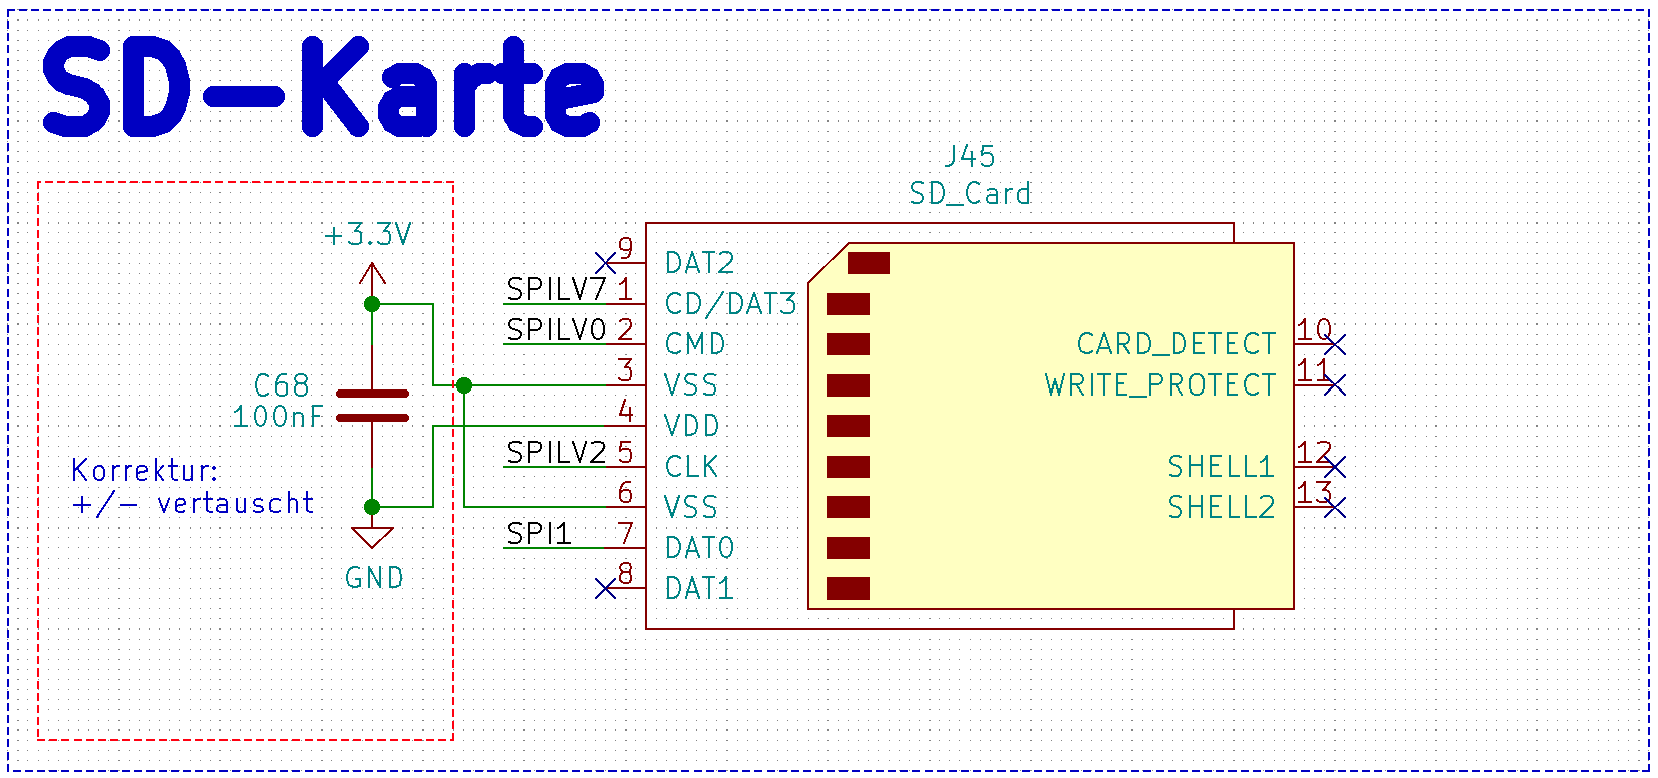
\includegraphics[width = 0.6 \textwidth]{graphics/Schema_SD_Karte}
\caption{Schema SD-Karte.}
\label{fig:Schema_SD_Karte}
\end{figure}

\paragraph{Funktionsbeschrieb der Schaltung}\mbox{}

In der Schaltung ist erkennbar, dass die SPI-Leitungen an die Pins des Adapters führen, genauso die Spannungsleitungen. Da die SD-Karte stets vom Mikrocontroller angesteuert wird, gibt es keine weiteren erwähnenswerte Funktionen zu beschreiben.